\chapter{Aufgabe}

Die Aufgabe bestand in einer Implementierung eines Webservices. Wir haben uns dabei für die Verwendung der Programmiersprache PHP entschieden. PHP hat den Vorteil, dass es auf nahezu jedem beliebigen Webserver ausführbar ist und relativ wenig Leistung benötigt. Dies wollen wir auch nach der Implementierung testen. Außerdem hatten wir uns für PHP entschieden, da wir gerne mal eine neue, uns eher unbekannte Programmiersprache kennenlernen wollten.
Als Framework haben wir uns für Slim\cite{slim} entschieden, ein Framework was sich vollständig auf die REST-Funktionalität beschränkt, trotzdem aber durch sogenannte Middlewares erweiterbar ist.
Als Zusatzaufgabe haben wir uns mit dem Thema Sicherheit befasst. Dafür sollte eine Authentifizierung mittels OAuth2\cite{oauth} implementiert werden und die Verschlüsselung durch HTTPS gelöst werden.

%Als Zusatzaufgabe sollte das Thema WS-Security durch Authentifizierung mittels OAuth2 und Verschlüsselung mittels HTTPS gelöst werden.

\chapter{Installation}
\section{Datenbank}
Für die Installation der Datenbank müssen die mitgelieferten Dumps bikesharingservice.sql und bikesharingservice\_oauth.sql in eine MySQL Datenbank eingefügt werden.
\begin{lstlisting}[caption={Datenbankimport}\label{lst:dbimport},captionpos=b] 
mysql -u root -p -h localhost
mysql> create database bikesharingservice;
mysql> create database bikesharingservice_oauth;
mysql> exit;
mysql -u username -p -h localhost bikesharingservice < bikesharingservice.sql
mysql -u username -p -h localhost bikesharingservice_oauth < 
	bikesharingservice_oauth.sql
\end{lstlisting}
Anschließend muss die Datenbank gestartet werden.
Eventuell muss in der php.ini die Zeile extension=pdo\_mysql.so einkommentiert werden.

Alternativ können die Datenbanken auch über phpMyAdmin importiert werden.

\section{Webservice und OAuth-Server}
Vorraussetzung für den Webservice und den OAuth-Server ist ein Webserver auf dem PHP und PDO installiert sind. In den beiden Dateien config.php und config\_oauth.php sind die Zugangsdaten für die Datenbank hinterlegt, diese müssen entsprechend angepasst werden. Anschließend kann der Order api einfach auf den Server kopiert werden. 
\section{Webclient}
Für den Webclient ist ebenfalls ein Server mit installiertem PHP nötig. Zusätzlich muss in der script.js die Variable baseURL durch die URL des Webservice ersetzt werden. In der head.php muss dies ebenfalls über die Variable \$api\_url geschehen. Durch die Variable \$oauth\_url wird zusätzlich der Link zum Authentifizierungsserver gesetzt.

\chapter{Webservice Endpoints}

Folgend eine Auflistung der möglichen Endpoints die in der API implementiert sind und über den Webservice abgerufen werden können. Einzelne Ressourcen werden nicht gesondert aufgelistet, sind aber bei allen GET-Requests jeweils über die ID möglich. Die Antfort ist sonst identisch, nur das ein einzelnes Element anstatt einer Liste zurückgegeben wird.

Die Auflistung soll die WADL ersetzen, da sich diese mit unserem verwendeten Framework nicht generieren lässt.

\begin{tabularx}{\columnwidth}{|X|p{1.5cm}|X|p{1.5cm}|}
	\hline
	Name & Method & URL & Access \\
	\hline
	\hline
	Alle verfügbare Fahrradstationen & GET & /stations & public \\
	\hline
	Spezielle Station & GET & /stations/stationID & public \\
	\hline
	Alle verfügbaren Fahrräder & GET & /bikes & public \\
	\hline
	Spezielles Fahrrad & GET & /bikes/bikesID & public \\
	\hline
	Alle Fahrradmodelle & GET & /models & public \\
	\hline
	Spezielles Fahrradmodell & GET & /models/modelID & public \\
	\hline
	Alle Buchungen & GET & /bookings & protected \\
	\hline
	Buchung erstellen & POST & /bookings & protected \\
	\hline
	Einzelne Buchung & GET & /bookings/bookingID & protected \\
	\hline
	Einzelne Buchung stornieren & DELETE & /bookings/bookingID & protected \\
	\hline
	Einzelne Buchung bearbeiten & PUT & /bookings/bookingID & protected \\
	\hline
	Accountinformationen & GET & /account & protected \\
	\hline
\end{tabularx}

In den folgenden Abschnitten werden diese Methoden genauer erklärt.

\section{GET Methoden}
\subsection{stations}
Liefert eine Liste aller verfügbaren Stationen zurück an denen Fahrräder
zum Verleih zur Verfügung stehen.

\begin{longtable}[c]{@{}lll@{}}
\toprule\addlinespace
Method & URL & Access
\\\addlinespace
\midrule\endhead
GET & /stations & public
\\\addlinespace
\bottomrule
\end{longtable}

\subsubsection{Parameter}\label{parameter}

\begin{longtable}[c]{@{}lll@{}}
\toprule\addlinespace
Name & Required & Description
\\\addlinespace
\midrule\endhead
location & nein & Standort an dem nach Stationen gesucht werden soll,
z.B. ``Dresden'' oder ``Berlin''
\\\addlinespace
model & nein & ID eines bestimmten Fahrradmodells nach dem gefiltert
werden soll, z.B. 105 oder 185
\\\addlinespace
\bottomrule
\end{longtable}

\subsubsection{Request Example}\label{request-example}

\begin{verbatim}
GET /stations?location=Dresden&model=105
\end{verbatim}

\subsubsection{Response}\label{response}

Liefert eine Liste von verfügbaren Stationen zurück, jede Station
besteht aus den folgenden Parametern: * stationId - Die einzigartige
Kennung der Station * name - Der Name der Station * longitude -
Längengrad * latitude - Breitengrad * bikes - Die Anzahl an zum Verleih
zur Verfügung stehenden Fahrräder in der Station * description - Die
ausführliche Beschreibung der Station * pictureUrl - Die URL eines Fotos
von der Station

\subsubsection{Response Examples}\label{response-examples}

\begin{verbatim}
{
   "stations" : [
      {
         "stationId" : 64,
         "name" : "Hauptbahnhof",
         "longitude" : -33.8670522,
         "latitude" : 151.1957362,
         "bikes" : 78,
         "description" : "Tolle Station am Hauptbahnhof, direkt vor dem Ausgang.",
         "pictureUrl" : "www.test.de/station64.jpg"
      },
      {
         "stationId" : 82,
         "name" : "Zoo",
         "longitude" : -33.8670522,
         "latitude" : 151.1957362,
         "bikes" : 108,
         "description" : "Eine Station direkt am Zoo.",
         "pictureUrl" : "www.test.de/station82.jpg"
      }
   ]
}
\end{verbatim}

\subsection{bikes}
Liefert eine Liste aller verfügbaren Fahrräder die zum Verleih zur
Verfügung stehen.

\begin{longtable}[c]{@{}lll@{}}
\toprule\addlinespace
Method & URL & Access
\\\addlinespace
\midrule\endhead
GET & /bikes & public
\\\addlinespace
\bottomrule
\end{longtable}

\subsubsection{Parameter}\label{parameter}

\begin{longtable}[c]{@{}lll@{}}
\toprule\addlinespace
Name & Required & Description
\\\addlinespace
\midrule\endhead
location & ja & Standort an dem nach verfügbaren Fahrrädern gesucht
werden soll, z.B. ``Dresden'' oder ``Berlin''
\\\addlinespace
radius & nein & Radius in dem um die location gesucht werden soll in
Meter (default: 2500), z.B. 5000
\\\addlinespace
modelId & nein & Die eindeutige Kennung eines bestimmten Fahrradmodells
nach dem gefiltert werden soll, z.B. 105 oder 185
\\\addlinespace
stationId & nein & Die eindeutige Kennung einer bestimmten
Verleihstation nach der gefiltert werden soll, z.B. 46 oder 4
\\\addlinespace
\bottomrule
\end{longtable}

\subsubsection{Request Example}\label{request-example}

\begin{verbatim}
GET /bikes?location=Dresden&radius=5000&modelId=105&stationId=4
\end{verbatim}

\subsubsection{Response}\label{response}

Liefert eine Liste von verfügbaren Fahrrädern, jedes Fahrrad besteht aus
den folgenden Parametern: * bikeId - Die einzigartige Kennung des
Fahrrads * modelId - Die einzigartige Kennung des Fahrradmodells * price
- Der Preis für 15 Minuten in Cent. * longitude - Längengrad * latitude
- Breitengrad * stationId - Falls das Fahrrad in einer Verleihstation
steht, ist dies die eindeutige Kennung der Station * distance - Die
Entfernung zum gewählten Standort

\subsubsection{Response Examples}\label{response-examples}

\begin{verbatim}
{
   "bikes" : [
      {
         "bikeId" : 46,
         "modelId" : 105,
         "price" : 100,
         "longitude" : -33.8670522,
         "latitude" : 151.1957362,
         "stationId" : 4,
         "distance": 2800
      },
      {
         "bikeId" : 34,
         "modelId" : 105,
         "price" : 150,
         "longitude" : -33.8670522,
         "latitude" : 151.1957362,
         "stationId" : 4 ,
         "distance": 2800
      }
   ]
}
\end{verbatim}

\subsection{models}
Liefert eine Liste aller verfügbaren Fahrradmodelle.

\begin{longtable}[c]{@{}lll@{}}
\toprule\addlinespace
Method & URL & Access
\\\addlinespace
\midrule\endhead
GET & /models & public
\\\addlinespace
\bottomrule
\end{longtable}

\subsubsection{Parameter}\label{parameter}

\begin{longtable}[c]{@{}lll@{}}
\toprule\addlinespace
Name & Required & Description
\\\addlinespace
\midrule\endhead
location & nein & Standort an dem nach verfügbaren Fahrrädern gesucht
werden soll, z.B. ``Dresden'' oder ``Berlin''
\\\addlinespace
stationId & nein & Die eindeutige Kennung einer bestimmten
Verleihstation nach der gefiltert werden soll, z.B. 46 oder 4
\\\addlinespace
\bottomrule
\end{longtable}

\subsubsection{Request Example}\label{request-example}

\begin{verbatim}
GET /models?location=Dresden&stationId=4
\end{verbatim}

\subsubsection{Response}\label{response}

Liefert eine Liste von verfügbaren Fahrradmodellen, jedes Modell besteht
aus den folgenden Parametern: * modelId - Die einzigartige Kennung des
Fahrradmodells * name - Der Name des Fahrradmodells * description - Eine
Beschreibung des Modells * pictureUrl - Die URL eines Fotos, welches das
Fahrradmodell zeigt * bikes - Die Anzahl an zum Verleih zur Verfügung
stehenden Fahrräder dieses Modells

\subsubsection{Response Examples}\label{response-examples}

\begin{verbatim}
{
   "models" : [
      {
         "modelId" : 105,
         "name" : "Rennrad",
         "description" : "Bestens geeignet für das Fahren auf dem Asphalt.",
         "pictureUrl" : "www.test.de/model105",
         "bikes" : 78
      },
      {
         "modelId" : 68,
         "name" : "Kinderfahrrad",
         "description" : "Geeignet für Kinder zwischen 6 und 9 Jahren.",
         "pictureUrl" : "www.test.de/model68",
         "bikes" : 8
      }
   ]
}
\end{verbatim}

\subsection{account}
Liefert die Accountinformationen des Nutzers.

\begin{longtable}[c]{@{}lll@{}}
\toprule\addlinespace
Method & URL & Access
\\\addlinespace
\midrule\endhead
GET & /account & protected
\\\addlinespace
\bottomrule
\end{longtable}

\subsubsection{Request Example}\label{request-example}

\begin{verbatim}
GET /account
\end{verbatim}

\subsubsection{Response}\label{response}

Liefert die Accountinformationen des Nutzers, ein Account besteht aus
den folgenden Parametern: * accountId - Die einzigartige Kennung des
Nutzers * email - Die E-Mail Adresse des Nutzers

\subsubsection{Response Examples}\label{response-examples}

\begin{verbatim}
{
   "accountId" : 1696,
   "email" : "test@test.com"
}
\end{verbatim}

\subsection{bookings}
Liefert eine Liste aller getätigten Buchungen.

\begin{longtable}[c]{@{}lll@{}}
\toprule\addlinespace
Method & URL & Access
\\\addlinespace
\midrule\endhead
GET & /bookings & protected
\\\addlinespace
\bottomrule
\end{longtable}

\subsubsection{Request Example}\label{request-example}

\begin{verbatim}
GET /bookings
\end{verbatim}

\subsubsection{Response}\label{response}

Liefert eine Liste aller getätigten Buchungen, jede Buchung besteht aus
den folgenden Parametern: * bookingId - Die einzigartige Kennung der
Buchung * bikeId - Die einzigartige Kennung des gebuchten Fahrrads *
date - Das Datum der Buchung

\subsubsection{Response Examples}\label{response-examples}

\begin{verbatim}
{
   "bookings" : [
      {
         "bookingId" : 1682,
         "bikeId" : 105,
         "date" : "2013-12-01 18:44:36"
      },
      {
         "bookingId" : 1696,
         "bikeId" : 168,
         "date" : "2013-12-01 18:45:24"
      }
   ]
}
\end{verbatim}

\section{POST Methoden}
\subsection{bookings}
Erstellt eine einzelne Buchung.

\begin{longtable}[c]{@{}lll@{}}
\toprule\addlinespace
Method & URL & Access
\\\addlinespace
\midrule\endhead
POST & /bookings & protected
\\\addlinespace
\bottomrule
\end{longtable}

\subsubsection{Request Example}\label{request-example}

\begin{verbatim}
POST /bookings
Params: {
   "id": 168
}
\end{verbatim}

\subsubsection{Parameter}\label{parameter}

\begin{longtable}[c]{@{}lll@{}}
\toprule\addlinespace
Name & Required & Description
\\\addlinespace
\midrule\endhead
id & ja & Die einzigartige Kennung des Fahrrads, z.B. 168
\\\addlinespace
\bottomrule
\end{longtable}

\subsubsection{Response}\label{response}

Liefert eine einzelne getätigte Buchung, die Buchung besteht aus den
folgenden Parametern: - 
\begin{itemize}
\item id - Die einzigartige Kennung der Buchung
\item bikeId - Die einzigartige Kennung des gebuchten Fahrrads
\item date - Der Zeitpunkt der Buchung
\end{itemize}

\subsubsection{Response Examples}\label{response-examples}

\begin{verbatim}
{
   	"bookingId" : 1696,
   	"bikeId" : 168,
   	"date" : "2013-12-01 18:45:24"
}
\end{verbatim}

\section{DELETE Methoden}
\subsection{bookings}
Storniert eine einzelne Buchung.

\begin{longtable}[c]{@{}lll@{}}
\toprule\addlinespace
Method & URL & Access
\\\addlinespace
\midrule\endhead
DELETE & /bookings/bookingId & protected
\\\addlinespace
\bottomrule
\end{longtable}

\subsubsection{Request Example}\label{request-example}

\begin{verbatim}
DELETE /bookings/1696
\end{verbatim}

\section{PUT Methoden}
\subsection{bookings}
Ändert eine einzelne Buchung.

WICHTIG: Content-Type: application/x-www-form-urlencoded

\begin{longtable}[c]{@{}lll@{}}
\toprule\addlinespace
Method & URL & Access
\\\addlinespace
\midrule\endhead
PUT & /bookings/bookingId & protected
\\\addlinespace
\bottomrule
\end{longtable}

\subsubsection{Request Example}\label{request-example}

\begin{verbatim}
PUT /bookings/bookingId
Params: {
   "bikeId": 168
}
\end{verbatim}

\subsubsection{Parameter}\label{parameter}

\begin{longtable}[c]{@{}lll@{}}
\toprule\addlinespace
Name & Required & Description
\\\addlinespace
\midrule\endhead
bikeId & nein & Die einzigartige Kennung des Fahrrads, z.B. 168
\\\addlinespace
\bottomrule
\end{longtable}

\subsubsection{Response}\label{response}

Liefert die geänderte Buchung, die Buchung besteht aus den folgenden
Parametern: - bookingId - Die einzigartige Kennung der Buchung - bikeId
- Die einzigartige Kennung des gebuchten Fahrrads - date - Der Zeitpunkt
an dem die Buchung getätigt wurde

\subsubsection{Response Examples}\label{response-examples}

\begin{verbatim}
{
   "bookingId" : 1696,
   "bikeId" : 168,
   "date" : "2013-12-01 18:45:24"
}
\end{verbatim}


\chapter{Webservice Implementierung}
Im Folgenden soll grundlegend erläutert werden wie sich ein Webservice mit dem Slim-Framwork implementieren lässt. Jeder Request wird dabei wie folgt entgegengenommen:
\begin{lstlisting}[caption={GET-Request mit Slim}\label{lst:slim},captionpos=b] 
$app->get('/bikes/:bikeId', function ($id) use ($app) {
   $query = "SELECT id, model, price, longitude, latitude, station 
	FROM bikes WHERE id = $id";
    echo getJsonObjectFromDb($query, $app); 
});
\end{lstlisting}
In dem Beispiel wird durch das Wort get festgelegt, dass GET-Requests entgegengenommen werden soll, durch das Ersetzen mit post, put oder delete, würden entsprechend die Arten von Requests entgegengenommen werden. Anschließend wird die URL definiert, wobei der Doppelpunkt angibt, dass es sich um eine Variable handelt. In der Funktion wird die SQL-Query erstellt und die von uns erstellte Funktion getJsonObjectFromDb() aufgerufen. Diese fürhrt die Query mittels PDO aus und liefert das Ergebnis als JSON zurück. Die Umwandlung des Ergebnisses in JSON erfolgt durch die PHP-Funktion json\_encode().

Auf die Art und Weise wurden alle Endpoints implementiert, zusätzliche Parameter lassen sich in der Funktion wie Folgt abrufen:
\begin{lstlisting}[caption={Paramater mit Slim}\label{lst:slim_param},captionpos=b] 
$app->request()->get('stationId');
\end{lstlisting}

\chapter{Webclient}

Der Webclient ist so konzipiert, dass prinzipiell auch mobile Endgeräte unterstützt werden.
Er bietet alle Funktionen die im vorhergehenden Kapitel beschrieben sind, zusätzlich sind diese im Folgenden noch einmal aufgelistet.
%Dazu zählen eine Suche, sowohl nach Adressen, als auch nach Ausleihstationen, eine Übersicht über die verfügbaren Fahrradmodelle und über die Stationen an denen Fahrräder ausgeliehen werden können.

\begin{figure}[h]
        \centering
	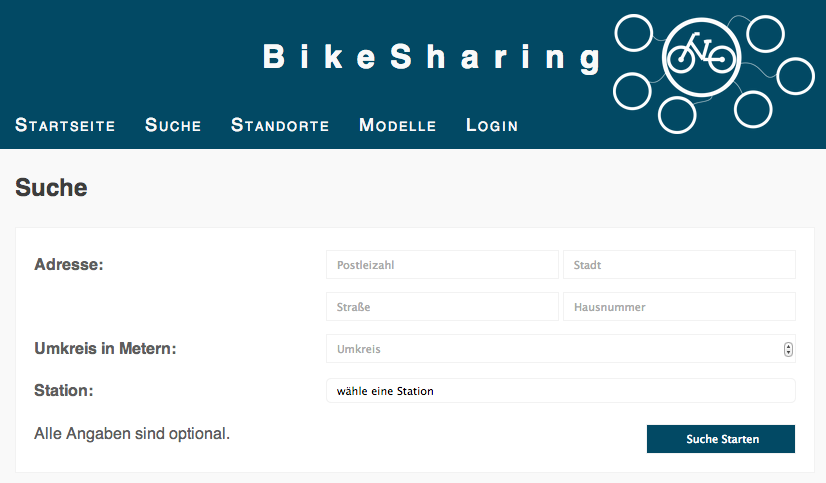
\includegraphics[height=80mm]{pics/bikesharing_search.png}
	\caption{Suche nach Fahrrädern}
\end{figure}

\begin{description}
	\item[Suche:] Es kann nach Fahrrädern an bestimmten Adressen oder Stationen gesucht werden. Nach dem Absenden der Suche werden alle gefundenen Fahrräder aufgelistet und jeweils die Entfernung zum angegebenen Standort angezeigt.
	\item[Stationen:] Alle Stationen werden zum einen in einer Liste, zum anderen auf einer Karte angezeigt. Beim Auswählen einer Station wird diese noch einmal im Detail angezeigt, inklusive dem Standort auf einer Karte und allen verfügbaren Fahrrädern.
	\item[Modelle:] Alle Modelle werden in einer Liste dargestellt. Beim Auswählen eines Modells wird dieses noch einmal im Detail angezeigt, inklusive allen verfügbaren Fahrrädern.
	\item[Profil:] Im Profil werden zum einen die Daten des Nutzern angezeigt, zum anderen alle getätigten Buchungen. Buchungen können hier auch storniert werden.
	\item[Fahrrad:] Für jedes Fahrrad existiert eine Detailansicht, wo das Modell und der Standort auf einer Karte angezeigt werden. Zusätzlich lässt sich hier das Fahrrad buchen.
\end{description}



\begin{figure}[h]
        \centering
	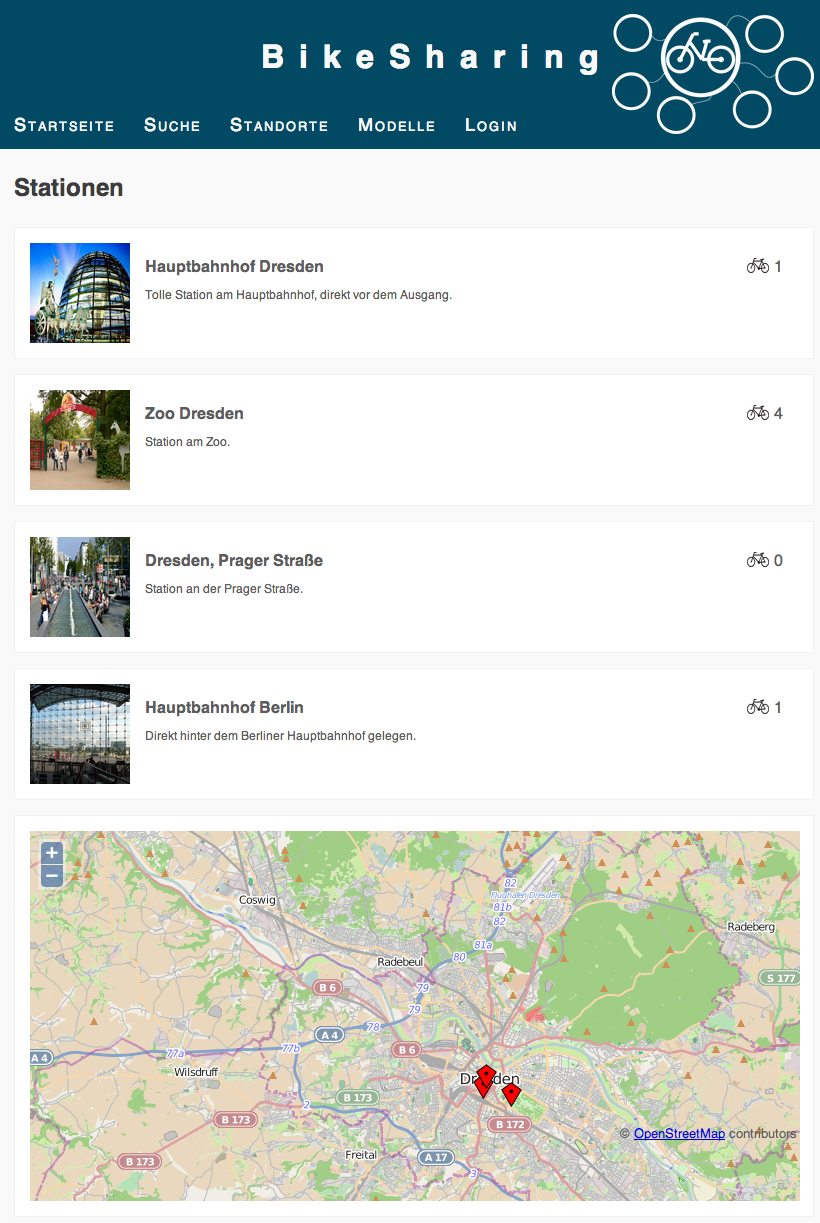
\includegraphics[height=180mm]{pics/bikesharing_stations.png}
	\caption{Liste aller verfügbaren Stationen}
\end{figure}

\chapter{Zusatzaufgabe Sicherheit}

%\section{OAuth2}
Wie in Abbildung \ref{oauth} dargestellt, besteht unser Webservice aus zwei Teilen. Neben der eigentlichen API, gibt es zusätzlich noch eine Komponente die für die Authentifizierung zuständig ist, den OAuth-Server. Dieser hat auch seine eigene Datenbank. Nachdem der Nutzer auf der Clientanwendung, in unserem Fall dem Webclient, auf eine Seite zugreifen möchte, die eine Authentifizierung erfordert, erfolgt eine Weiterleitung zum OAuth-Server. Dort muss der Nutzer sich dann mit seinen Zugangsdaten anmelden und bestätigen, dass die Clientanwendung auf die privaten Daten zugreifen darft. Daraufhin wird der Nutzer wieder zum Webclient weitergeleitet und dabei die Authenfication-Code übergeben, der vom OAuth-Server generiert wurde. Diesen Code verwendet die Clientanwendung zusammen mit ihren eigenen Zugangsdaten um beim OAuth-Server einen Access-Token anzufordern. Mit diesem Access-Token kann die Clientanwendung nun auf die privaten Daten des Nutzers zugreifen.

Um zu verhindern das Unautorisiere Personen den Access-Token abgreift, wird für die komplette Kommunikation HTTPS verwendet. Zusätzlich erfolgen alle Abfragen an den Webservice direkt vom Server des Webclient aus, der Access-Token wird dort in der Session gespeichert. Dadurch ist die unsichere clientseitige Speicherung mit JavaScript nicht nötig.

\begin{figure}[h]
        \centering
	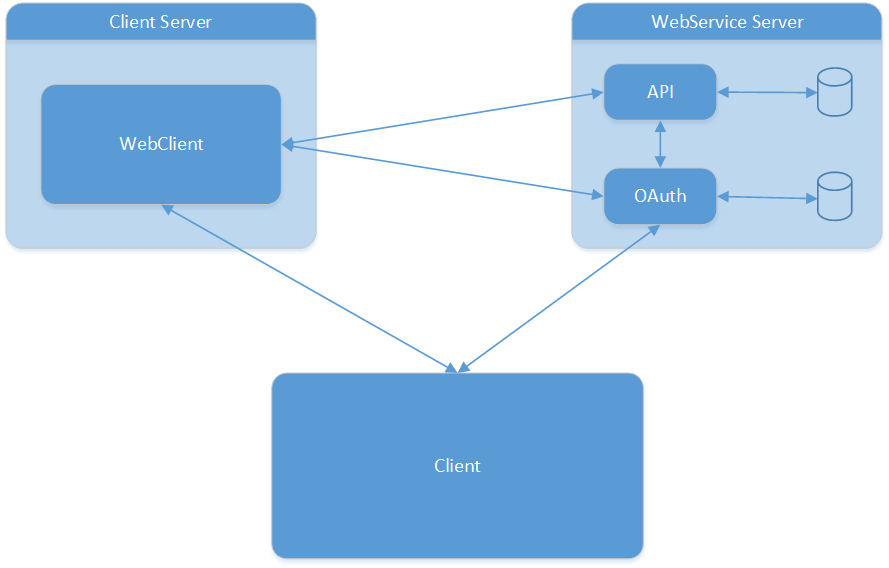
\includegraphics[height=70mm]{pics/Architektur.png}
	\caption{Kommunikation zwischen, Webservice, Client und Nutzer}
\end{figure}\label{oauth}

%\section{Implementierung}

\chapter{Fazit}

Die Implementierung des Webclient ist nach Vorlage einer durchdachten API gut machbar.

Das Slim-Framework war eine gute Wahl, da die Verwendung sehr einfach und fehlerfrei verlief. Die Implementierung eines OAuth-Servers ist recht zeitaufwendig und umständlich, vor allem wenn man sich damit bisher noch nicht befasst hat. Leider hat auch die OAuth-Middleware für das Slim-Framework nicht funktioniert, sodass eine eigene Lösung gefunden werden musste, um die Authentifizierung auf dem Webservice zu kontrollieren.

Der Aufwand ist, ja nach gewählter Aufgabe, recht hoch, insbesondere wenn man, wie in diesem Fall, Programmiersprachen wählt, die den Teammitgliedern gar nicht, oder nur rudimentär geläufig sind.

Wie am Anfang geplant, konnten wir unsere Anwendung nach der Entwicklung problemlos auf einem fast kostenlosem Webserver testen und sie ließ sich dort direkt ohne Probleme ausführen, es war keine besondere Einrichtung erforderlich. 

%Wir hatten uns für PHP entschieden, da PHP den Vorteil bringt, dass es auf nahezu jedem beliebigen Webserver ausführbar ist und relativ wenig Leistung benötigt. Wir konnten unsere Anwendung nach der Entwicklung problemlos auf einem fast kostenlosem Webserver testen und sie ließ sich dort direkt ohne Probleme ausführen, es war keine besondere Einrichtung erforderlich. Außerdem hatten wir uns für PHP entschieden, da wir gerne mal eine neue, uns eher unbekannte Programmiersprache kennenlernen wollten.

\bibliography{literatur}

